An important feature for a framework is acceptance testing. Anonymous evaluation was done. Participants were used to evaluate the quality of the framework and check if the goals
to create an easy to use and simple framework were achieved. The participants were presented with tutorial\cite{tut} for the framework, 
each of them had to have basic knowledge in programming. The choice of first to fourth year students presented a good study group since it presented people
with different levels of programming experience. The participants had to asses the quality of the 
tutorial, understanding of the framework and usability of the GUI. Each had to answer the following questions\cite{monkey}:

\begin{enumerate}
\item How helpful was it to understand the basics of the framework?
\item How complex was it to create the first examples?
\item How complex was to create the advanced example?
\item How far on the tutorial did you reach in 30 minutes?
\end{enumerate}
 
Second part of the evaluation participants had to asses the graphical user interface by answering the following questions: 

\begin{enumerate}
\item How intuitive is it?
\item How simple is it?
\item Were there enough options presented?
\item Can you give additional feedback that can help improve the GUI?
\end{enumerate}

SurveyMonkey was used for creating the survey. Through the evaluation the following problems in the GUI and the tutorial were identified and fixed:

\textbf{Graphical User Interface}
\begin{itemize}
\item Omitting \textit{http} should still create a valid URL.
\item If no arguments are provided an error message should pop up
\item There should be help text for the \textit{terminals} field to specify its format.
\end{itemize}

\textbf{Tutorial}
\begin{itemize}
\item There should be a link to the libraries/frameworks websites?
\item The version of each library/framework should be specified?
\item There should be more frequent code examples?
\end{itemize}

As seen in the results from the survey, participants had hard time with running the first example as seen in fig \ref{fig:firstex}. This was due to the multiple dependencies of the
framework, lack of installation script and ambiguity in the tutorial. However
in the end of the tutorial there was a high number participants that understood the basic framework functionality. Most of the participants managed to complete the tutorial
in less than 30 minutes, however these 30 minutes didn't include set up time.

\begin{figure}[htp]
\centering
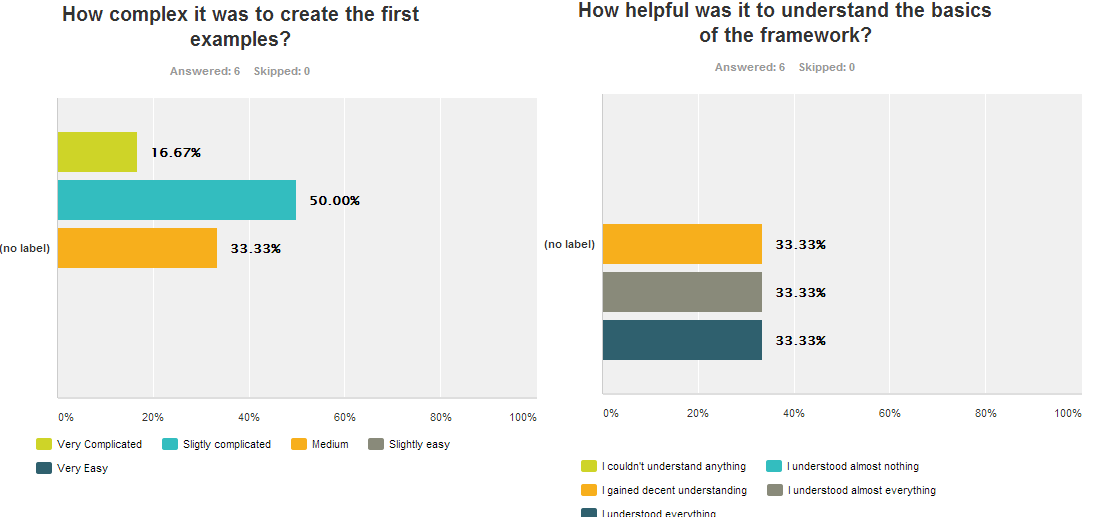
\includegraphics[scale=0.5]{Figures/q1.png}
\caption{Plotted answers to the question: "How complex it was to create the first examples?" and "How helpful was it to understand the basics of the framework?" }
\label{fig:firstex}
\end{figure}

For the GUI the results from participants were quite positive. The main problems with the GUI were the lack of feedback in the case of an error and lack of automation
at the URL fields. Each of those problems was fixed by adding pop-up dialogues in case of a missing field, example for the \textit{Terminals} field was added and the
URL fields don't require \textit{http://} in front of the host name.